% --- Placeholder for figures (replace with actual image inclusion) ---
\newcommand{\imageplaceholder}[3][0.8\textwidth]{%
    \begin{figure}[ht]
    \centering
    \fbox{\parbox{#1}{
      \centering
      \textbf{Image Placeholder: #2} \\ \vspace{2mm}
      #3 \\ \vspace{2mm}
    }}
    \caption{#2}
    \label{fig:#3}
    \end{figure}
}

% Configure graphicx path (adjust relative path as needed from main.tex location)
% Assuming main.tex is in the root, and images are in src/images/CHAPTER_FOLDER/
\graphicspath{{src/images/}} % Simplified path for example

\chapter{Classical Cryptography}\label{chap:classical_crypto}

Classical cryptography covers the rich history and the foundational techniques developed to secure communications long before the advent of quantum computers posed a significant threat. This chapter traces the evolution of these cryptographic methods, explains the core principles that underpin modern classical systems, and details the workings of symmetric and asymmetric encryption, hash functions, and digital signatures. By understanding this classical foundation, we can better appreciate its vulnerabilities to quantum attacks, setting the stage for later discussions on quantum-resistant solutions.

\section{Historical Development of Cryptography}
The practice of secret communication, or cryptography, has evolved over millennia, constantly adapting to meet military, diplomatic, and commercial demands for confidentiality \parencite{kahn1996codebreakers, singh1999code}. Its journey began in \textbf{Ancient Origins}, featuring early methods like non-standard Egyptian hieroglyphs, secret Mesopotamian formulas, and the Spartan scytale (around 400 BCE), a simple transposition cipher device \parencite{madness2020classical}. The subsequent \textbf{Classical Period} witnessed the emergence of more structured systems, including the Caesar cipher and more sophisticated substitution methods like the Vigenère cipher, designed to thwart basic frequency analysis. For example, the Caesar cipher replaces each letter $P$ with $C = (P + k) \pmod{26}$, where $k$ is the shift. For $k=3$, $A \to D$, $B \to E$, etc. Techniques operating on multiple letters simultaneously, such as the Playfair and Hill ciphers, also appeared \parencite{singh1999code, stallings2017cryptography}. This progression led to the \textbf{Mechanical Era} of the early 20th century, exemplified by complex electromechanical devices like the Enigma machine, which automated intricate polyalphabetic substitutions \parencite{singh1999code}. Notably, the successful cryptanalysis of Enigma significantly spurred early computing efforts. The \textbf{Modern Era} of cryptography was catalyzed by Claude Shannon's groundbreaking information theory in 1949 \parencite{shannon1949communication}, the development of digital computers, and the move towards standardization, beginning with the Data Encryption Standard (DES) in 1977 \parencite{nist1999des}. This era firmly established Kerckhoffs's Principle – the idea that a cryptosystem's security should depend solely on the secrecy of the key, not the algorithm itself \parencite{kerckhoffs1883}. It also saw a fundamental paradigm shift with the invention of public-key cryptography in 1976 \parencite{diffie1976new}, revolutionizing key management and enabling digital signatures.

\begin{figure}[ht]
    \centering
    % Make sure the path is correct relative to where main.tex is located
    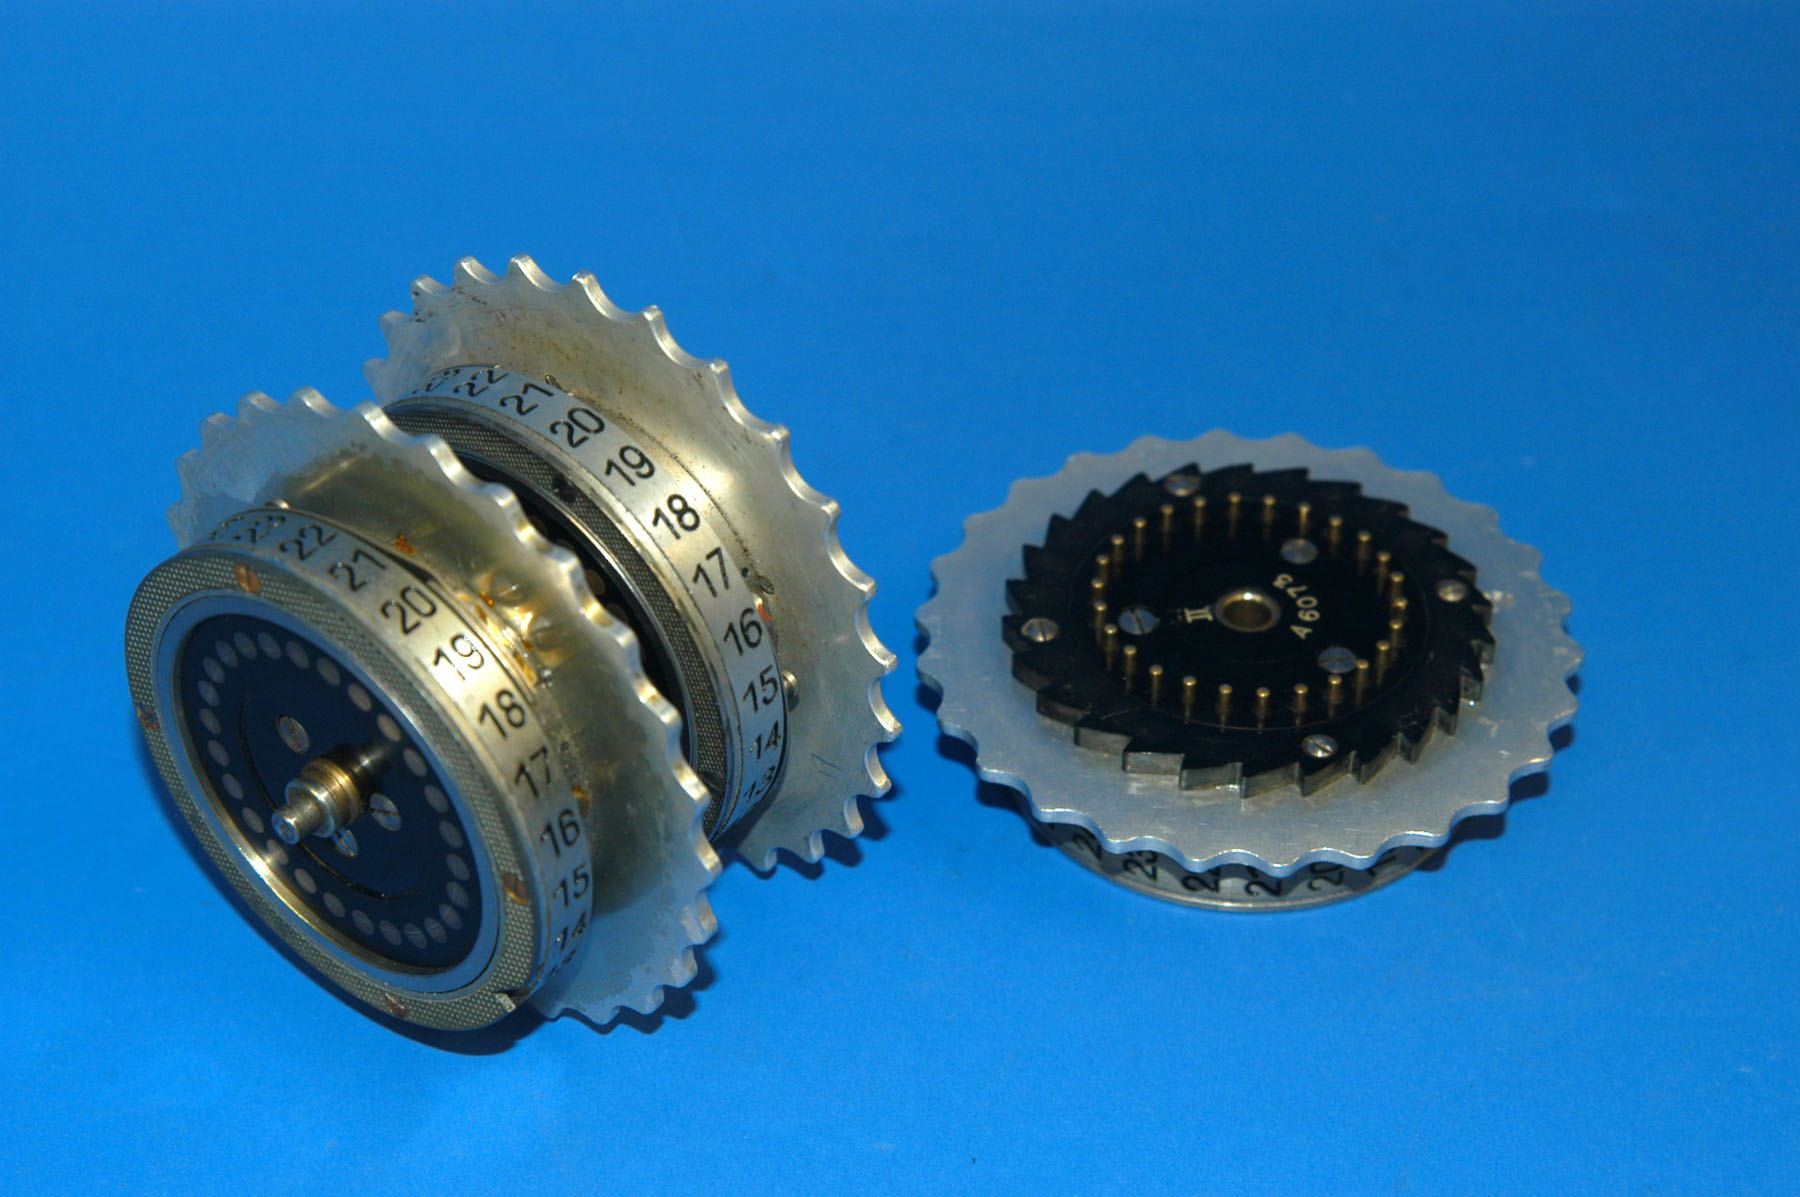
\includegraphics[width=0.8\textwidth]{03_Classical_Cryptography/enigma_rotors}
    \caption{Internal mechanism of the Enigma machine showing the rotor system that provided complex, changing polyalphabetic substitution.}
    \label{fig:enigma_rotors_ch3}
\end{figure}

\section{Fundamentals of Modern Cryptography}\label{sec:crypto_fundamentals_ch3}

Modern classical cryptography aims to provide strong security guarantees based on rigorous mathematical principles, operating under the assumption that adversaries possess only classical computing capabilities.

\subsection{Core Security Goals}
Well-designed cryptographic systems are built to achieve several essential security objectives \parencite{katz2014introduction, stallings2017cryptography}. Primarily, they ensure \textbf{Confidentiality}, preventing unauthorized access to information, typically achieved through encryption. They also guarantee \textbf{Integrity}, ensuring that data has not been tampered with undetected, often using hash functions or Message Authentication Codes (MACs). Furthermore, \textbf{Authentication} serves to verify the origin of data or the identity of communicating parties, usually accomplished with MACs or digital signatures. Finally, \textbf{Non-repudiation} prevents a sender from falsely denying having sent a message; this is a key feature provided by digital signatures, which rely on public-key cryptography.

\subsection{Mathematical Foundations}
The security of most modern cryptosystems rests on the assumed \textbf{Computational Hardness} of certain mathematical problems for \textit{classical} computers \parencite{katz2014introduction}. This means specific problems, like factoring very large integers, are believed to require an infeasible amount of time or computational resources for any classical algorithm to solve. Cryptography cleverly leverages functions based on these hard problems. \textbf{One-way Functions} are easy to compute in one direction but computationally difficult to reverse; cryptographic hash functions are a prime example. A crucial special category is \textbf{Trapdoor Functions}: these are one-way functions that become easy to invert if, and only if, specific secret information (the "trapdoor") is known. Trapdoor functions form the mathematical bedrock of public-key encryption schemes. It is vital to remember that this "hardness" assumption is relative to the computational model—specifically, classical computers—and, as we will see, may not hold against the power of quantum computation. A function $f: X \to Y$ is \textbf{one-way} if $f(x)$ is easy to compute for any $x \in X$, but for most $y$ in the image, it is hard to find $x$ such that $f(x) = y$. A \textbf{trapdoor function} $f_k$ is one-way unless you know a secret trapdoor $t$, in which case inversion is easy. For example, multiplying large primes is easy, but factoring is hard.

\section{Symmetric Key Cryptography}\label{sec:symmetric_key_ch3}

Symmetric cryptography, also known as secret-key cryptography, employs a single, shared secret key for both the encryption and decryption processes. Its main advantages are speed and efficiency, making it highly suitable for encrypting large volumes of data. However, its primary operational challenge lies in the secure distribution and management of this shared secret key among the communicating parties \parencite{katz2014introduction}.

\subsection{Operations and Security}
Modern symmetric algorithms, such as the Advanced Encryption Standard (AES), typically achieve strong security by applying multiple rounds of combined operations. These rounds often involve \textbf{Substitution}, frequently implemented using S-boxes (Substitution boxes), which replaces data elements in a complex, non-linear way to obscure the relationship between the plaintext, the key, and the ciphertext. This process contributes to the property of *confusion*. Algorithms also employ \textbf{Permutation}, which rearranges the order of data elements, spreading the influence of individual plaintext bits across many ciphertext bits, thus achieving *diffusion*. Both confusion and diffusion work together to thwart statistical attacks. Additionally, sophisticated \textbf{Key Scheduling} algorithms generate unique subkeys, or "round keys," derived from the main secret key for use in each distinct round of the encryption or decryption process.

The security level of a symmetric cipher against a brute-force attack (systematically trying every possible key) is primarily determined by the length of the key, denoted by $n$. A key of length $n$ bits defines a key space of $2^n$ possible keys. Therefore, the classical security level, measured in bits, is approximately equal to the key length:
\begin{equation}\label{eq:key_space_ch3}
    \text{Classical Security Level (bits)} \approx n = \log_2(\text{Key Space Size})
\end{equation}
However, it's crucial to note that this theoretical strength can be significantly undermined by flaws in the implementation rather than the algorithm itself. Systems can be vulnerable to \textbf{side-channel attacks}, such as timing analysis \parencite{kocher1996timing} or power analysis \parencite{mangard2007power}. These attacks exploit information leaked through observable physical characteristics of the computation (like execution time or power consumption patterns) to deduce information about the secret key, bypassing the need to break the mathematical structure of the cipher directly.

Block ciphers like AES are built as Substitution-Permutation Networks (SPNs), applying rounds of S-boxes (nonlinear substitution), permutations, and key mixing. The key space size is $2^n$ for an $n$-bit key, so brute-force requires $O(2^n)$ operations. Grover's quantum algorithm reduces this to $O(2^{n/2})$.

\subsection{Block Ciphers and Modes}
Common symmetric algorithms include block ciphers, which operate on fixed-size blocks of data. \textbf{DES (Data Encryption Standard)}, the former standard with a 56-bit key, is now considered insecure primarily due to its small key size, making it vulnerable to brute-force attacks with modern hardware. Its successor, \textbf{AES (Advanced Encryption Standard)} \parencite{nist2001aes}, is the current global standard. AES supports key sizes of 128, 192, or 256 bits and is widely considered secure against all practical classical attacks when implemented correctly.

Because block ciphers process data in fixed chunks, encrypting messages larger than a single block requires a \textbf{Mode of Operation} (e.g., CBC, CTR, GCM \parencite{nist_sp800_38d}). These modes define how to repeatedly apply the block cipher's operation to sequential blocks of data, providing essential properties like error propagation control, parallelism, or even combining confidentiality with data integrity and authenticity in what are known as Authenticated Encryption with Associated Data (AEAD) modes, like AES-GCM. The incorrect choice or flawed implementation of an operation mode can introduce severe vulnerabilities, even when using a strong underlying block cipher like AES.

\begin{figure}[ht]
    \centering
    % Add images tux_ecb.png and tux_cbc.png to illustrate
    \includegraphics[width=0.45\textwidth]{03_Classical_Cryptography/tux_ecb}
    \includegraphics[width=0.45\textwidth]{03_Classical_Cryptography/tux_cbc}
    \caption{ECB mode (left) reveals patterns; CBC mode (right) obscures them.}
    \label{fig:ecb_vs_cbc}
\end{figure}

\subsection{Quantum Impact on Symmetric Keys}
While symmetric key cryptography is not broken by Shor's algorithm in the same way as public-key systems, it is impacted by Grover's quantum search algorithm \parencite{grover1996fast}. Grover's algorithm offers a quadratic speedup for unstructured search problems, which includes the problem of finding a secret key by brute force. This effectively halves the security level in bits against a quantum attacker: an $n$-bit symmetric key provides approximately $n/2$ bits of security against a quantum brute-force search. Consequently, to maintain a security level equivalent to 128 bits in the post-quantum era (a common benchmark), stronger keys like AES-256 (providing $256/2 = 128$ bits of quantum security) are recommended \parencite{bernstein2017post, nist_pqc}.

\begin{figure}[ht]
    \centering
    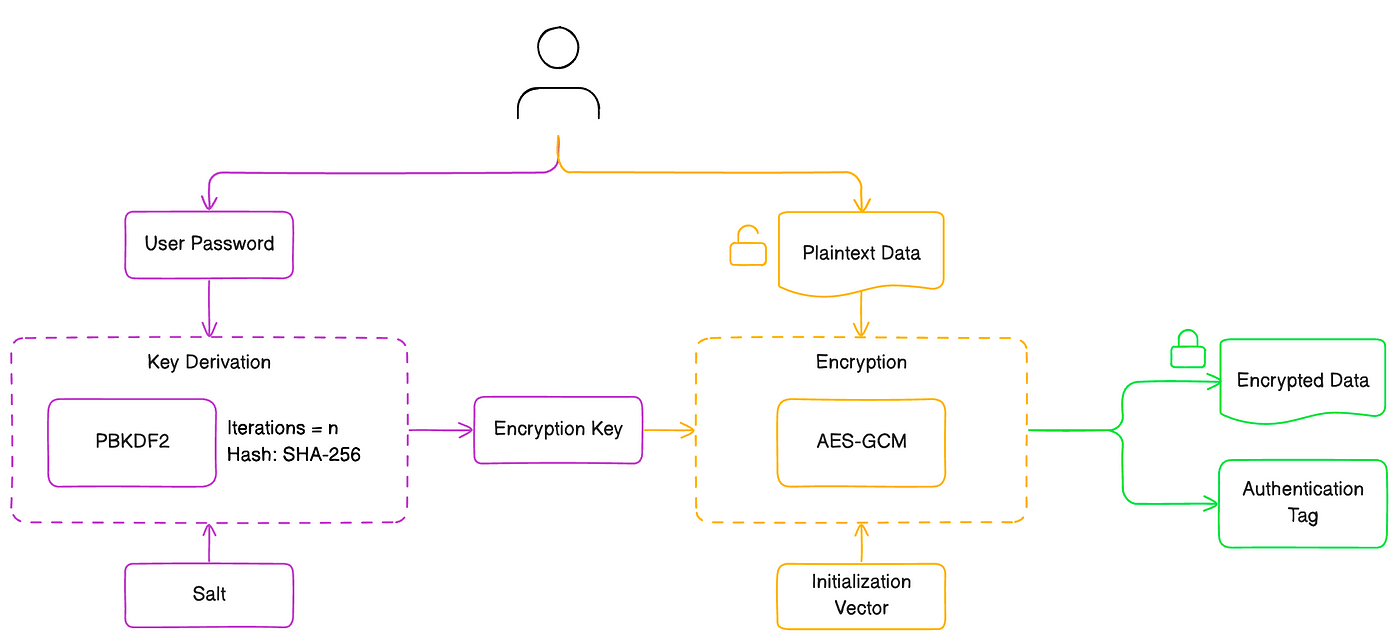
\includegraphics[width=0.9\textwidth]{03_Classical_Cryptography/aes_gcm_workflow}
    \caption{AES-GCM authenticated encryption workflow, providing both confidentiality via CTR mode and integrity/authentication via GHASH.}
    \label{fig:aes_gcm_ch3}
\end{figure}

\section{Public Key Cryptography}\label{sec:public_key_ch3}

Introduced in the seminal 1976 paper by Diffie and Hellman \parencite{diffie1976new}, public-key (or asymmetric) cryptography represented a revolutionary departure from traditional symmetric systems. It utilizes a pair of mathematically related keys: a \textbf{public key}, which can be distributed widely without compromising security, and a corresponding \textbf{private key}, which must be kept secret by its owner. The public key is typically used for encrypting messages or verifying digital signatures, while the private key is used for decryption or creating signatures. This ingenious two-key structure elegantly solves the key distribution problem inherent in symmetric cryptography and provides the foundation for digital signatures. The security of widely deployed public-key systems relies on the presumed computational difficulty of certain mathematical problems for classical computers.

\subsection{RSA Algorithm}\label{subsec:rsa_ch3}
The RSA algorithm, named after its inventors Rivest, Shamir, and Adleman \parencite{rivest1978method}, derives its security from the practical difficulty of factoring the product of two very large prime numbers. An RSA key pair consists of a public key $(n, e)$ and a private key $(n, d)$. Here, $n$ is the modulus, calculated as the product of two large, secret prime numbers $p$ and $q$ ($n=pq$). The public exponent $e$ and private exponent $d$ are chosen such that they satisfy the mathematical relationship $ed \equiv 1 \pmod{\phi(n)}$, where $\phi(n) = (p-1)(q-1)$ is Euler's totient function. Encryption of a message $M$ (represented as an integer) involves computing the ciphertext $C = M^e \bmod n$. Decryption uses the private key exponent $d$ to recover the original message: $M = C^d \bmod n$.

\textbf{Key Generation:}
\begin{enumerate}
    \item Choose primes $p, q$; $n = pq$.
    \item $\phi(n) = (p-1)(q-1)$.
    \item Choose $e$ coprime to $\phi(n)$.
    \item Find $d$ such that $ed \equiv 1 \pmod{\phi(n)}$.
\end{enumerate}
\textbf{Example:} $p=11, q=13, n=143, \phi(n)=120, e=7, d=103$. Encrypt $M=5$: $C=5^7 \bmod 143=117$. Decrypt: $M=117^{103} \bmod 143=5$.

Classically, the security of RSA hinges on the assumption that factoring the large modulus $n$ into its prime components $p$ and $q$ is computationally infeasible. Current cryptographic guidelines recommend RSA key sizes (the bit length of $n$) of at least 2048 or 3072 bits to provide adequate security against classical attacks \parencite{nist_sp800_57p1r5}. However, RSA faces a catastrophic \textbf{Quantum Threat} from Shor's algorithm \parencite{shor1994algorithms}. Shor demonstrated that a sufficiently powerful quantum computer could factor large integers in polynomial time, meaning it could efficiently find $p$ and $q$ given $n$, and subsequently derive the private key $d$ from the public key $(n, e)$. This capability completely breaks the RSA cryptosystem, regardless of the key size used \parencite{bernstein2017post}. Beyond the quantum threat, RSA implementations must also guard against \textbf{Implementation Attacks}. Vulnerabilities such as padding oracle attacks (famously demonstrated by Bleichenbacher \parencite{bleichenbacher1998chosen}) or various side-channel attacks can compromise RSA security if the system is not implemented carefully using standardized padding schemes (like OAEP) and countermeasures against physical information leakage.

\begin{figure}[h]
    \centering
    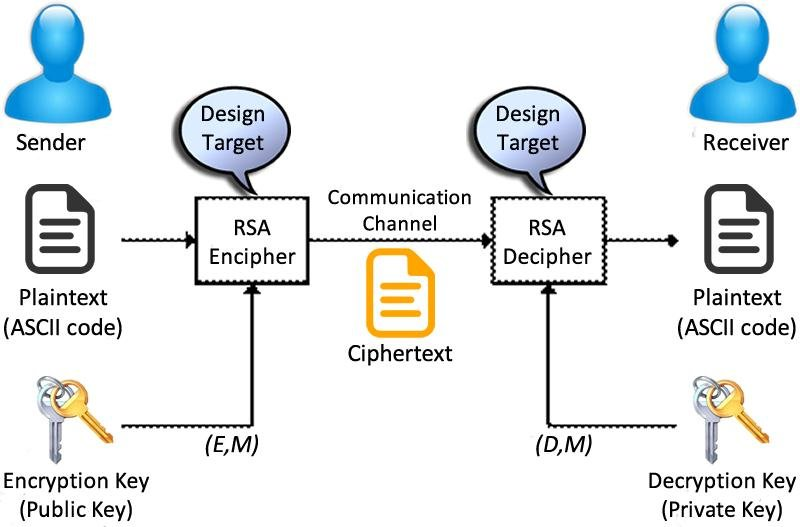
\includegraphics[width=0.8\textwidth]{03_Classical_Cryptography/rsa_encryption}
    \caption{RSA encryption (using public key) and decryption (using private key) process. Security relies on the difficulty of factoring $n$.}
    \label{fig:rsa_encryption_ch3}
\end{figure}

% Placeholder figure retained from original text
\imageplaceholder{Classical vs Quantum Factoring Complexity}{Graph comparing exponential/sub-exponential classical complexity vs polynomial quantum (Shor) complexity for factoring.}{shor_vs_classical_complexity}

\subsection{Elliptic Curve Cryptography (ECC)}\label{subsec:ecc_ch3}
Elliptic Curve Cryptography (ECC), independently proposed by Koblitz \parencite{koblitz1987elliptic} and Miller \parencite{miller1985use}, offers public-key cryptographic primitives with security comparable to RSA but using significantly smaller key sizes. ECC's security is based on the difficulty of the Elliptic Curve Discrete Logarithm Problem (ECDLP). The primary \textbf{Advantages} of ECC stem from this key size efficiency: smaller keys lead to faster computations, lower power consumption, and reduced bandwidth and storage requirements. This makes ECC particularly suitable for resource-constrained environments such as mobile devices, smart cards, and Internet of Things (IoT) sensors. For instance, a 256-bit ECC key is generally considered to offer a similar level of classical security to a 3072-bit RSA key \parencite{nist_sp800_57p1r5}. ECC operations involve arithmetic with points on a carefully chosen elliptic curve defined over a finite field.

An elliptic curve over $\mathbb{F}_p$ is $y^2 \equiv x^3 + ax + b \pmod{p}$, $4a^3+27b^2 \not\equiv 0$. Point addition: $m = (y_2-y_1)(x_2-x_1)^{-1} \pmod{p}$ for $P \neq Q$; $m = (3x_1^2+a)(2y_1)^{-1} \pmod{p}$ for $P=Q$. $x_3 = m^2-x_1-x_2$, $y_3 = m(x_1-x_3)-y_1$.

\imageplaceholder[0.7\textwidth]{Elliptic Curve Point Addition}{Geometric interpretation of $P+Q=R$ on an elliptic curve.}{ecc_addition_ch3_math}

Its \textbf{Classical Security} relies on the belief that the ECDLP is computationally hard for classical algorithms. While secure against classical computers, ECC faces the same critical \textbf{Quantum Threat} as RSA. Shor's algorithm can be adapted to efficiently solve the ECDLP on a quantum computer, thus rendering standard ECC-based systems (including ECDH key exchange and ECDSA signatures) insecure in the presence of capable quantum attackers \parencite{bernstein2017post}.

% Placeholder figure retained from original text (commented out)
%\begin{figure}[ht]
%    \centering
%    \includegraphics[width=0.7\textwidth]{03_Classical_Cryptography/elliptic_curve_addition}
%    \caption{Geometric interpretation of point addition on an elliptic curve, fundamental to ECC operations.}
%    \label{fig:ecc_addition_ch3}
%\end{figure}

\subsection{Diffie-Hellman Key Exchange (DH)}\label{subsec:dh}
The Diffie-Hellman (DH) protocol is a foundational cryptographic method that enables two parties, often referred to as Alice and Bob, to establish a shared secret key over an insecure communication channel, even if an eavesdropper intercepts all their messages \parencite{diffie1976new}. Remarkably, they can achieve this without having any prior shared secrets. The process begins with Alice and Bob publicly agreeing on a large prime number $p$ and a generator $g$ (an integer whose powers modulo $p$ generate a large subgroup). Alice then chooses a secret integer $a$, computes her public value $A = g^a \bmod p$, and sends $A$ to Bob. Similarly, Bob chooses a secret integer $b$, computes his public value $B = g^b \bmod p$, and sends $B$ to Alice. Upon receiving the other's public value, Alice computes the shared secret $S = B^a \bmod p = (g^b)^a \bmod p = g^{ab} \bmod p$. Bob independently computes $S = A^b \bmod p = (g^a)^b \bmod p = g^{ab} \bmod p. Both arrive at the same secret value $S = g^{ab} \bmod p$, which is difficult for an eavesdropper to compute knowing only $p, g, A,$ and $B$.

Public: $p, g$. Alice: $a$, $A=g^a \bmod p$. Bob: $b$, $B=g^b \bmod p$. Shared secret: $S=g^{ab} \bmod p$. Security: DLP and CDH.

The \textbf{Classical Security} of the DH protocol relies on the presumed difficulty of the Computational Diffie-Hellman (CDH) problem (computing $g^{ab} \bmod p$ given $g, g^a \bmod p, g^b \bmod p$) and the underlying Discrete Logarithm Problem (DLP) (computing $a$ given $g$ and $g^a \bmod p$). A significant practical \textbf{Vulnerability} of the basic DH protocol is its susceptibility to Man-in-the-Middle (MitM) attacks if the exchanged public values ($A$ and $B$) are not authenticated. An attacker could intercept $A$ and $B$, substitute their own values, and establish separate secret keys with Alice and Bob, relaying messages between them while reading or modifying them. This necessitates using DH within authenticated protocols like TLS or authenticating the exchanged values using digital signatures. The \textbf{Quantum Threat} to DH is severe: Shor's algorithm can efficiently solve the DLP \parencite{shor1994algorithms}, allowing a quantum attacker to compute the secret exponents $a$ and $b$ from the public values $A$ and $B$, thus deriving the shared secret $S$. Elliptic Curve Diffie-Hellman (ECDH), which performs the key exchange using points on an elliptic curve and relies on the ECDLP, faces the exact same quantum vulnerability.

% Placeholder figure retained from original text
\imageplaceholder{Diffie-Hellman Key Exchange}{Diagram illustrating the DH key exchange process (mathematical steps or paint mixing analogy).}{diffie_hellman_exchange}

\section{Hash Functions}\label{sec:hash_functions_ch3}

Cryptographic hash functions are indispensable tools in modern cryptography. They take an input message of arbitrary length and produce a fixed-size output string, commonly known as a hash digest or hash value \parencite{menezes1996handbook}. Think of them as creating a unique "digital fingerprint" for data. They are fundamental components for ensuring data integrity, securely storing passwords (by hashing them before storage), and constructing digital signatures and message authentication codes.

\subsection{Required Properties}
To be considered cryptographically secure, a hash function $H(x)$ must satisfy three essential properties:
\begin{enumerate}
    \item \textbf{Pre-image Resistance:} Given a hash output $h$, it must be computationally infeasible to find \textit{any} input $x$ such that $H(x)=h$. (It's hard to find the original message given only its hash).
    \item \textbf{Second Pre-image Resistance:} Given a specific input $x_1$, it must be computationally infeasible to find a \textit{different} input $x_2 \neq x_1$ such that $H(x_1) = H(x_2)$. (It's hard to find another message that hashes to the same value as a given message).
    \item \textbf{Collision Resistance:} It must be computationally infeasible to find \textit{any pair} of distinct inputs $x_1 \neq x_2$ such that $H(x_1) = H(x_2)$. (It's hard to find any two different messages that produce the same hash output). This is generally the strongest property and implies second pre-image resistance.
\end{enumerate}

\subsection{Algorithms and Security}
Several families of hash functions have been developed and standardized over time. Older standards like \textbf{MD5 and SHA-1} are now considered broken due to the discovery of practical collision attacks, meaning pairs of different inputs producing the same hash can be found with feasible effort. Consequently, they should no longer be used for security purposes \parencite{stallings2017cryptography}. The \textbf{SHA-2} family, which includes widely used variants like SHA-256 and SHA-512, is the current workhorse standard and is considered secure against known classical attacks. The \textbf{SHA-3} family, based on the Keccak algorithm selected through a public NIST competition, offers a different internal structure (known as a "sponge construction") compared to SHA-2, providing valuable algorithmic diversity \parencite{nist_fips202}. Additionally, high-performance modern functions like \textbf{BLAKE2 and BLAKE3} offer strong security guarantees alongside very high speeds \parencite{blake3}.

\begin{figure}[ht]
    \centering
    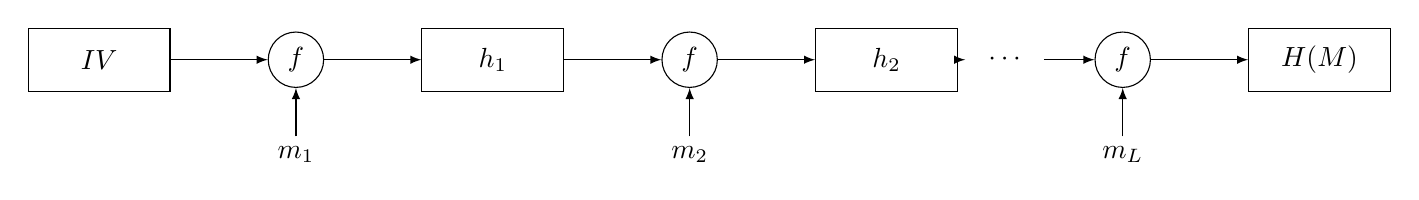
\begin{tikzpicture}[
        box/.style={draw, minimum width=1.8cm, minimum height=0.8cm},
        circ/.style={draw, circle, minimum size=0.7cm},
        >=latex
    ]
        % Initial value and blocks with more space between components
        \node[box] (iv) at (0,0) {$IV$};
        \node[circ] (f1) at (2.5,0) {$f$};
        \node[box] (h1) at (5,0) {$h_1$};
        \node[circ] (f2) at (7.5,0) {$f$};
        \node[box] (h2) at (10,0) {$h_2$};
        \node at (11.5,0) {$\cdots$};
        \node[circ] (f3) at (13,0) {$f$};
        \node[box] (h3) at (15.5,0) {$H(M)$};
        
        % Message inputs with consistent spacing
        \node (m1) at (2.5,-1.2) {$m_1$};
        \node (m2) at (7.5,-1.2) {$m_2$};
        \node (m3) at (13,-1.2) {$m_L$};
        
        % Arrows with consistent spacing
        \draw[->] (iv) -- (f1);
        \draw[->] (m1) -- (f1);
        \draw[->] (f1) -- (h1);
        \draw[->] (h1) -- (f2);
        \draw[->] (m2) -- (f2);
        \draw[->] (f2) -- (h2);
        \draw[->] (h2) -- (11,0);
        \draw[->] (12,0) -- (f3);
        \draw[->] (m3) -- (f3);
        \draw[->] (f3) -- (h3);
    \end{tikzpicture}
    \caption{Merkle-Damgård construction: the compression function $f$ iteratively processes message blocks $m_i$ with the previous hash value to produce the final hash $H(M)$.}
    \label{fig:merkle_damgard}
\end{figure}

Regarding the \textbf{Quantum Impact}, Grover's algorithm \parencite{grover1996fast} can be applied to speed up the search for preimages and potentially collisions. For preimages, it reduces the effective security from $n$ bits to $n/2$ bits for an $n$-bit hash output. For collision resistance, the classical "birthday attack" takes roughly $O(2^{n/2})$ steps, while certain quantum algorithms might find collisions in roughly $O(2^{n/3})$ steps. More generally, applying Grover's search for collisions effectively takes $O(2^{n/2})$ quantum steps. Because quantum attacks weaken the effective security, using hash functions with larger output sizes, such as SHA-256, SHA-384, or SHA-512, is recommended to maintain adequate security margins in the post-quantum era \parencite{bernstein2017post}.

\section{Digital Signatures and PKI}\label{sec:digital_signatures_pki_ch3}

Digital signatures are a critical mechanism in secure digital communication, providing strong assurances of \textbf{Authentication} (verifying the sender's identity), \textbf{Integrity} (ensuring the message content hasn't been altered after signing), and \textbf{Non-repudiation} (preventing the sender from credibly denying having sent the signed message). They achieve these goals by ingeniously combining asymmetric cryptography with cryptographic hash functions. The typical signing process involves the sender first computing a hash digest of the message ($H(M)$). Then, the sender uses their \textit{private} key ($d$) to apply a signing operation (which is related to decryption in algorithms like RSA) to this hash, producing the digital signature ($S = \text{Sign}(H(M), d)$). The signature $S$ is then typically appended to the message $M$. Verification is performed by anyone who receives the message and signature. The verifier uses the sender's \textit{public} key to apply a verification operation (related to encryption in RSA) to the signature $S$ and compares the result to a freshly computed hash of the received message $M$. If they match, the signature is considered valid, confirming the message's authenticity and integrity.

Signing: $S=\text{Sign}_{K_{priv}}(H(M))$. Verification: $\text{Verify}_{K_{pub}}(S) \stackrel{?}{=} H(M)$.

\subsection{Public Key Infrastructure (PKI)}
The entire security premise of digital signatures hinges on the verifier's ability to trust that the public key they are using genuinely belongs to the claimed sender. How can this trust be established and managed at scale? \textbf{Public Key Infrastructure (PKI)} provides the necessary framework, policies, and procedures to enable secure management and use of public keys \parencite{stallings2017cryptography}. At the core of PKI are trusted third parties known as \textbf{Certificate Authorities (CAs)}. CAs issue \textbf{digital certificates}, which are electronic documents that securely bind an identity (like a person's name, an organization, or a website's domain name) to a specific public key. These certificates are themselves digitally signed by the CA using its own private key, allowing users to verify the certificate's authenticity using the CA's trusted public key. PKI also includes mechanisms to handle situations where a certificate needs to be invalidated before its natural expiration date (e.g., if the corresponding private key is compromised). This is typically done through \textbf{Certificate Revocation Lists (CRLs)} or the \textbf{Online Certificate Status Protocol (OCSP)}. This structured trust system enables secure communication and transactions across large networks like the internet, underpinning technologies like HTTPS/TLS for secure web browsing.

The \textbf{Quantum Threat to Signatures} is substantial because the most commonly used digital signature algorithms today (such as RSA-PSS and ECDSA) are based on the same asymmetric cryptographic primitives (RSA and ECC) that are vulnerable to Shor's algorithm. A sufficiently powerful quantum computer could potentially derive the private signing key from the publicly available verification key (the public key contained in the certificate). This would allow an attacker to forge signatures that appear legitimate, completely undermining the authentication and non-repudiation guarantees \parencite{bernstein2017post}. Hash-based signatures, which rely only on the security of hash functions, represent one category of quantum-resistant alternatives that address this vulnerability.

\begin{figure}[ht]
    \centering
    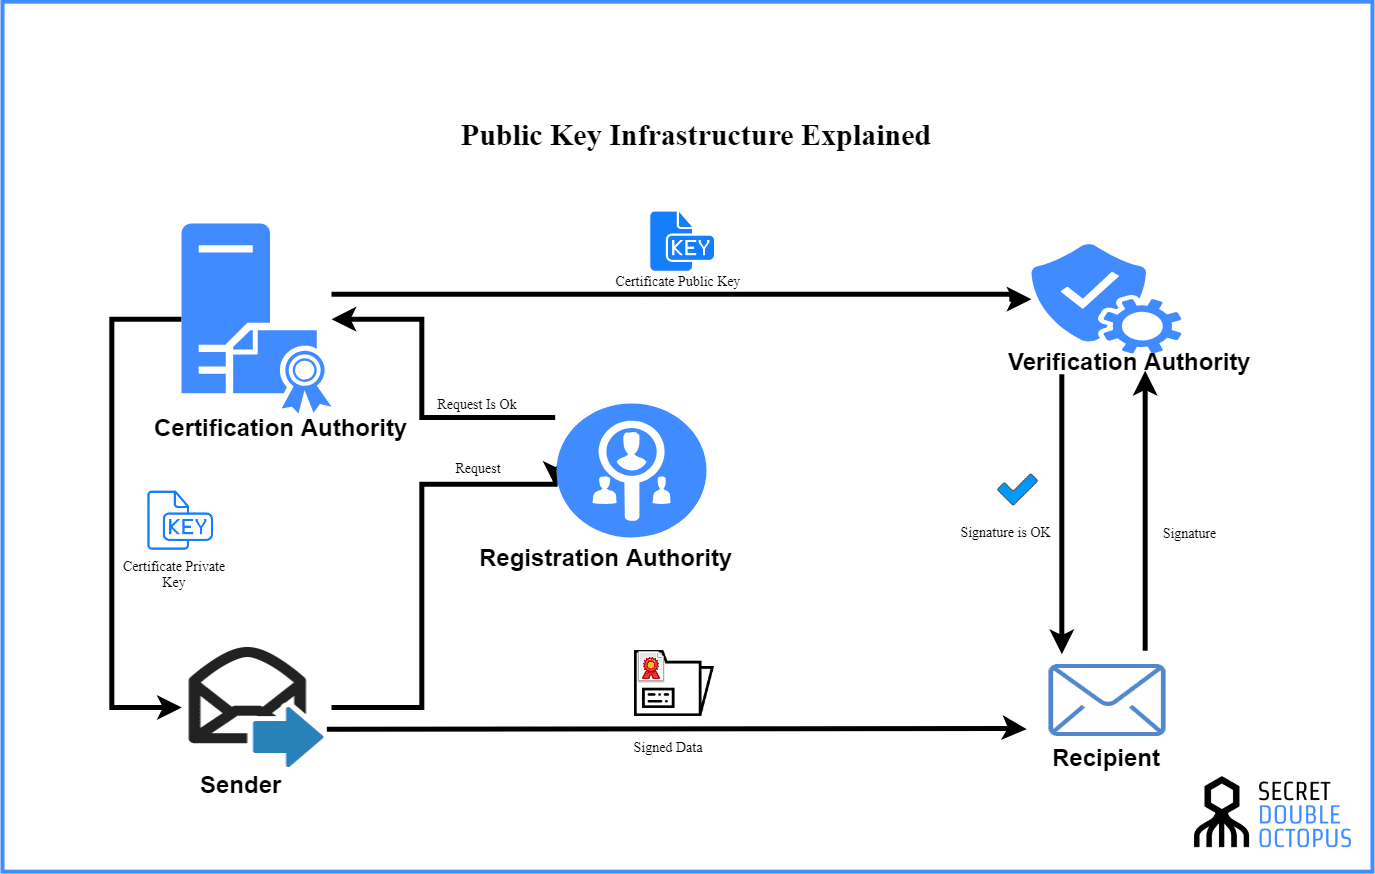
\includegraphics[width=0.8\textwidth]{03_Classical_Cryptography/pki_trust_model}
    \caption{Public Key Infrastructure (PKI) trust model showing Certificate Authorities (CAs) issuing certificates to bind identities to public keys.}
    \label{fig:pki_model_ch3}
\end{figure}

\section{Security Foundations: The Classical Achilles' Heel}\label{sec:security_foundations_ch3}

As highlighted throughout this chapter, the security guarantees of widely deployed classical public-key cryptography fundamentally depend on \textbf{computational hardness assumptions}. These are well-defined mathematical problems believed to be intractable—too difficult to solve in any practical amount of time—for adversaries who are restricted to using only classical computing resources \parencite{katz2014introduction}. The most critical of these underlying hard problems are the \textbf{Integer Factorization Problem (IFP)}, upon which RSA's security rests; the \textbf{Discrete Logarithm Problem (DLP)}, which secures Diffie-Hellman key exchange and related systems like DSA; and the \textbf{Elliptic Curve Discrete Logarithm Problem (ECDLP)}, the foundation for ECC and its derivatives (ECDH, ECDSA). For decades, these problems have provided a solid foundation for security, as the best-known classical algorithms to solve them require computational effort that grows exponentially or sub-exponentially with the size of the keys, making them practically unsolvable for sufficiently large key sizes.

Classical algorithms for IFP, DLP, ECDLP are super-polynomial or exponential; Shor's quantum algorithm solves them in polynomial time $O(\text{poly}(\log N))$.

However, this entire classical foundation is precisely what is shattered by the advent of quantum computing, specifically by Shor's algorithm. As mentioned previously, Shor's algorithm provides a way to solve IFP, DLP, and ECDLP in polynomial time on a quantum computer. This means that the very mathematical problems chosen for their classical difficulty become efficiently solvable with the right quantum hardware, rendering these cornerstone classical public-key cryptosystems insecure. This represents the core quantum challenge to classical cryptography.

\section{Protocol Design and Implementation Security}\label{sec:protocol_design_ch3}

Building truly secure systems requires significantly more than just selecting strong cryptographic algorithms; it demands the design of secure \textbf{protocols} that carefully orchestrate how these cryptographic primitives are used together \parencite{stallings2017cryptography}. Even if the underlying algorithms like AES or RSA are theoretically sound, subtle flaws in the protocol design can introduce critical vulnerabilities. For instance, failing to properly authenticate the public key exchange messages in the basic Diffie-Hellman protocol leaves it wide open to Man-in-the-Middle (MitM) attacks, completely negating the security goals.

Furthermore, errors made during the \text{implementation} phase—how the algorithms and protocols are actually coded and deployed—can be equally devastating. These \textbf{Implementation Vulnerabilities} can manifest in various ways. Improper handling of data formatting and padding, especially in systems like RSA, can lead to "padding oracle" attacks (like Bleichenbacher's attack on older SSL/TLS versions \parencite{bleichenbacher1998chosen}), which allow attackers to decrypt messages or forge signatures without solving the underlying hard mathematical problem. Another significant class of implementation flaws involves information leakage through \textbf{side channels}. Attackers might observe physical characteristics of the device performing cryptographic operations, such as minute variations in computation time (timing attacks \parencite{kocher1996timing}) or fluctuations in power consumption (power analysis \parencite{mangard2007power}), and use this leaked information to deduce secret keys \parencite{boneh2020graduate}. These side-channel attacks often bypass the theoretical security of the algorithm entirely. Therefore, secure protocol design combined with careful, robust, and often constant-time implementation practices are absolutely critical for achieving meaningful security in real-world systems.

% Placeholder figure retained from original text
\imageplaceholder{Side-Channel Attack Concept}{Conceptual diagram showing information leakage (power, timing) during crypto operations.}{side_channel_attack_concept}

\section{Conclusion: The Classical Foundation and the Quantum Challenge}

Classical cryptography provides the essential toolkit that has secured our digital world for decades. This toolkit includes efficient symmetric ciphers like AES for ensuring the confidentiality of bulk data, versatile asymmetric systems like RSA and ECC for managing keys securely and providing digital signatures, and robust hash functions like SHA-2 and SHA-3 for verifying data integrity. The security architecture of this entire classical framework is fundamentally built upon the assumption that certain specific mathematical problems are computationally intractable for classical computers.

However, as this chapter has outlined, this classical foundation faces an existential challenge from the potential advent of large-scale quantum computing. The threat is twofold: \textbf{Shor's algorithm} directly targets the core public-key cryptosystems (RSA, Diffie-Hellman, ECC and their derivatives) by efficiently solving the hard mathematical problems (IFP, DLP, ECDLP) upon which their security relies. This effectively breaks these systems entirely. Simultaneously, \textbf{Grover's algorithm} weakens the security of symmetric ciphers and hash functions by providing a quadratic speedup for search-based attacks, necessitating the use of longer keys and hash outputs to maintain equivalent security levels \parencite{bernstein2017post, mosca2018cybersecurity}. This looming quantum threat mandates a fundamental shift in our approach to cryptography. It drives the urgent need to develop, standardize, and ultimately transition to new cryptographic solutions—collectively known as \textbf{post-quantum cryptography (PQC)}—which are specifically designed to resist attacks from both powerful classical computers and anticipated future quantum computers. The nature and characteristics of these PQC solutions will be explored in subsequent chapters.